\documentclass[oneside,a4paper,14pt]{extarticle}
\usepackage[T1,T2A]{fontenc}
\usepackage[
a4paper,
top=2cm,
bottom=2cm,
left=2.5cm,
right=1.5cm
]{geometry}
\usepackage[utf8]{inputenc}
\usepackage[russian]{babel}
\usepackage{textcomp}
\usepackage{indentfirst}
\usepackage{listings}
\usepackage{listingsutf8}
\usepackage{xcolor}
\usepackage{float}
\usepackage{enumitem}
\usepackage{graphicx}
\usepackage{mwe}
\usepackage{wrapfig}
\usepackage{caption}
\usepackage{amsmath}
\usepackage{amsfonts}
\usepackage{amsthm}
\usepackage[all]{xy}
\usepackage[breaklinks]{hyperref}
\usepackage{titlesec}

\titleformat{\section}{\normalfont\normalsize\bfseries}{\thesection}{1em}{}
\titleformat{\subsection}{\normalfont\normalsize\bfseries}{\thesubsection}{1em}{}
\titleformat{\subsubsection}{\normalfont\normalsize\bfseries}{\thesubsubsection}{1em}{}

\renewcommand\baselinestretch{1.33}
\setlength{\parindent}{1.25cm}

\lstset{
	language=Python,
	basicstyle=\ttfamily\small,
	keywordstyle=\color{blue},
	commentstyle=\color{green!60!black},
	stringstyle=\color{red},
	numbers=left,
	numberstyle=\tiny\color{gray},
	frame=single,
	breaklines=true,
	showstringspaces=false,
	tabsize=2,
	inputencoding=cp1251,
	extendedchars=true,
}
\begin{document}
	\newpage\thispagestyle{empty}
	\begin{center}
		МИНИСТЕРСТВО НАУКИ И ВЫСШЕГО ОБРАЗОВАНИЯ\\
		РОССИЙСКОЙ ФЕДЕРАЦИИ\\
		ФЕДЕРАЛЬНОЕ ГОСУДАРСТВЕННОЕ БЮДЖЕТНОЕ\\
		ОБРАЗОВАТЕЛЬНОЕ УЧРЕЖДЕНИЕ ВЫСШЕГО ОБРАЗОВАНИЯ\\
		«ВЯТСКИЙ ГОСУДАРСТВЕННЫЙ УНИВЕРСИТЕТ»\\
		Институт математики и информационных систем\\
		Факультет автоматики и вычислительной техники\\
		Кафедра электронных вычислительных машин
	\end{center}
	\vspace{20mm}
	\begin{center}
		Отчёт по лабораторной работе №6\\
		по дисциплине\\
		<<Промпт-инжиниринг>>\\
		<<Проектирование комплексного промпта для мультимодальной генерации>>\\
		<<Вариант 29>>\\
	\end{center}
	\vspace{48mm}
	\noindent
	Выполнил студент гр. ИВТб-1303-06-00 \hfill \rule[-0.5mm]{30mm}{0.15mm}\,/Шубин В.Ю./\\[0.5cm]
	Проверил доцент кафедры ЭВМ \hfill \rule[-0.5mm]{30mm}{0.15mm}\,/Колупаев А.В./
	\vfill
	\begin{center}
		Киров\\
		2026
	\end{center}
	\newpage
	\thispagestyle{empty}
	\section*{Введение}
	\noindent
	\textbf{Цель работы:} Формирование системного навыка проектирования мультимодальных генеративных конвейеров (пайплайнов), позволяющих автоматизировать создание минимально жизнеспособных продуктов (MVP) на основе индустриальных кейсов. Освоение методологии <<быстрого прототипирования>> (Rapid Prototyping), при которой инженер управляет нейросетями для последовательной генерации технической документации, визуальных активов и программного кода.
	\textbf{Языковые модели, используемые в работе:}
	\begin{itemize}
		\item \textbf{DeepSeek Chat} --- генерация ТЗ, текстов интерфейса, дизайн-системы, Python-кода;
		\item \textbf{DALL-E 3} --- генерация логотипа, изображений;
		\item \textbf{Qwen} --- валидация и итеративная коррекция промптов.
	\end{itemize}
	\textbf{Предметная область варианта 29:} Генератор тестовых данных (Test Data Generator)\\
	\textbf{Роль А (Разработчик):} Настраивает параметры генерации (объем, типы полей, распределение), ожидает мгновенный предпросмотр и экспорт в стандартных форматах. Характер: технически подкован, ценит скорость и точность.\\
	\textbf{Роль Б (Система):} Имитирует работу ETL-конвейера, формирует структурированные датасеты с реалистичными значениями, валидирует типы данных, предоставляет визуальный предпросмотр таблицы.\\
	\textbf{Фоновая сцена:} Веб-интерфейс в темной теме (Dark Mode), акцент на читаемость табличных данных, моноширинные шрифты, четкая сетка элементов управления.
	\newpage
	\section*{Задание 1: Архитектурный анализ и генерация Технического Задания}
	\noindent
	\textbf{Цель:} Научиться использовать возможности больших языковых моделей в роли системного архитектора для глубокого анализа предметной области, обоснованного выбора технологий быстрого прототипирования и формирования детального Технического Задания, адаптированного под дальнейшую автоматическую кодогенерацию.
	\subsection*{1.1 Системный промпт Архитектора}
	\lstinputlisting[language=]{1.nonutf.txt}
	\subsection*{1.2 Журнал выбора технологий (Tree of Thoughts)}
	\noindent
	Фрагмент ответа модели с анализом альтернатив:
	\noindent
	\textbf{Вариант 1: CLI-утилита на Python (argparse + CSV)}\\
	-- Плюсы: минимальные зависимости, высокая скорость генерации, легко интегрировать в CI/CD.\\
	-- Минусы: отсутствие визуального предпросмотра, неудобно для ручного тестирования и настройки параметров.
	\noindent
	\textbf{Вариант 2: Jupyter Notebook с интерактивными виджетами (ipywidgets)}\\
	-- Плюсы: привычная среда для Data Scientists, наглядный вывод данных.\\
	-- Минусы: требует установки Jupyter, сложен в деплое как самостоятельный MVP, медленная отрисовка таблиц при >500 строк.
	\noindent
	\textbf{Вариант 3: Веб-дашборд на Streamlit (Python + Pandas)}\\
	-- Плюсы: нативная поддержка таблиц (st.dataframe), боковая панель конфигурации, встроенный экспорт, быстрый запуск, адаптивность.\\
	-- Минусы: требует локального сервера для демонстрации.
	\noindent
	\textbf{Вывод:} Выбран \textbf{Вариант 3 (Streamlit + Pandas)}.\\
	\textbf{Обоснование:} Идеальный баланс между скоростью разработки MVP и интерактивностью. Позволяет реализовать симуляцию <<загрузки конвейера>> через st.spinner, поддерживает прямое скачивание CSV/JSON и корректно отображает большие таблицы.
	\newpage
	\subsection*{1.3 Итоговое Техническое Задание}
	\lstinputlisting[language=]{2.nonutf.txt}
	\subsection*{1.4 Валидация шаблона}
	\noindent
	Для проверки универсальности промпт был протестирован на описании <<Генератор SQL-скриптов для миграций>>. Структура ТЗ сохранилась, изменились только сущности и форматы вывода. Шаблон успешно абстрагируется от предметной области и применим к любым DevTools-инструментам.
	\newpage
	\section*{Задание 2: Генерация мультимедийного наполнения и визуальных ресурсов}
	\noindent
	\textbf{Цель:} Научиться проектировать комплексные цепочки промптов для создания согласованного набора текстовых и графических материалов, которые визуально и смыслово соответствуют техническому заданию.
	\subsection*{2.1 Описание дизайн-системы}
	\noindent
	Промпт для генерации дизайн-системы:
	\lstinputlisting[language=]{3.nonutf.txt}
	\newpage
	\noindent
	Ответ модели (фрагмент):\\
	\begin{tabular}{|l|l|l|}
		\hline
		\textbf{Элемент} & \textbf{Описание} & \textbf{Hex-код} \\ \hline
		Основной фон & Темный технический & \#121420 \\ \hline
		Карточки/панели & Глубокий серый & \#1E2130 \\ \hline
		Акцентный цвет & Инженерный циан & \#00D4FF \\ \hline
		Таблица (строки) & Чередование оттенков & \#232738 / \#2A2F45 \\ \hline
		Успех/валидация & Неоновый зеленый & \#10B981 \\ \hline
		Основной текст & Светло-серый & \#E2E8F0 \\ \hline
		Второстепенный текст & Приглушенный & \#94A3B8 \\ \hline
	\end{tabular} \\
	\noindent
	\textbf{Типографика:} Заголовки: Inter Medium 18-22px. Данные таблиц: JetBrains Mono Regular 14px.\\
	\textbf{Тональность:} Сухая, техническая, без лишних пояснений, ориентированная на инженеров.
	\subsection*{2.2 Галерея ассетов}
	\noindent
	Тексты интерфейса (JSON):
	\lstinputlisting[language=]{4.nonutf.txt}
	\newpage
	\noindent
	Промпт для логотипа (DALL-E 3):
	\begin{lstlisting}
		Minimalist tech logo for data generation tool, isometric cube transforming into structured grid rows, 
		dark background #121420, cyan accent lines #00D4FF, clean geometric style, developer aesthetic, 
		1024x1024, transparent background.
	\end{lstlisting}
	\begin{figure}[H]
		\centering
		
\includegraphics[width=17cm]{1.png}
		\caption{Сгенерированный логотип приложения}
	\end{figure}
	\newpage
	\noindent
	Промпт для иконки конфигурации:
	\begin{lstlisting}
		Flat UI icon for data configuration, gear merged with database cylinder, 
		dark theme, cyan highlight #00D4FF, minimal flat design, 256x256, transparent background.
	\end{lstlisting}
	\begin{figure}[H]
		\centering
		
\includegraphics[width=13cm]{2.png}
		\caption{Иконка панели настроек}
	\end{figure}
	\noindent
	Промпт для иконки экспорта:
	\begin{lstlisting}
		Simple export icon, downward arrow above layered documents, 
		cyan and green accents, dark background, modern tech style, 256x256, transparent background.
	\end{lstlisting}
	\begin{figure}[H]
		\centering
		
\includegraphics[width=13cm]{3.png}
		\caption{Иконка экспорта данных}
	\end{figure}
	\newpage
	\subsection*{2.3 Эволюция стиля}
	\noindent
	Исходная генерация статусных сообщений содержала излишне дружелюбные формулировки (<<Готово! Вот ваши прекрасные данные!>>). После добавления в промпт директивы <<использовать лаконичный технический стиль, избегать эмоциональных окрасок, использовать терминологию Data Engineering>> модель выдала исправленный вариант (<Генерация завершена. Валидация типов пройдена>>).
	\newpage
	\section*{Задание 3: Мультимодальная генерация кода и сборка интерфейса}
	\noindent
	\textbf{Цель:} Научиться конструировать комплексные системные промпты, которые позволяют автоматизировать процесс разработки ПО, объединяя структурированные технические требования и подготовленный мультимедийный контент в функциональный прототип.
	\subsection*{3.1 Комплексный промпт Разработчика}
	\lstinputlisting[language=]{5.nonutf.txt}
	\subsection*{3.2 Журнал визуальной отладки (Self-Correction Log)}
	\begin{table}[H]
		\centering
		\begin{tabular}{|c|p{4cm}|p{5cm}|p{3.5cm}|}
			\hline
			\textbf{№} & \textbf{Проблема} & \textbf{Промпт коррекции} & \textbf{Результат} \\ \hline
			1 & Таблица выходила за границы контейнера & <<Оберни st.dataframe в st.container(border=True) и задай max-height через custom CSS>> & Таблица скроллится внутри карточки \\ \hline
			2 & Данные генерировались мгновенно, без задержки & <<Оберни логику генерации в st.spinner("⏳ Инициализация ETL-конвейера..."). Добавь time.sleep(1.5)>> & Реализована имитация обработки \\ \hline
			3 & Кнопка экспорта не работала после перегенерации & <<Используй st.session_state для хранения df. Привяжи download_button к состоянию>> & Экспорт сохраняет актуальные данные \\ \hline
			4 & Цвета полей ввода не соответствовали темной теме & <<Примени custom CSS для input[type="number"], select: border: 1px solid #334155; background: #1E2130>> & UI полностью соответствует Style Guide \\ \hline
		\end{tabular}
		\caption{Итерации отладки кода}
	\end{table}
	\subsection*{3.3 Финальный результат}
	\begin{figure}[H]
		\centering
		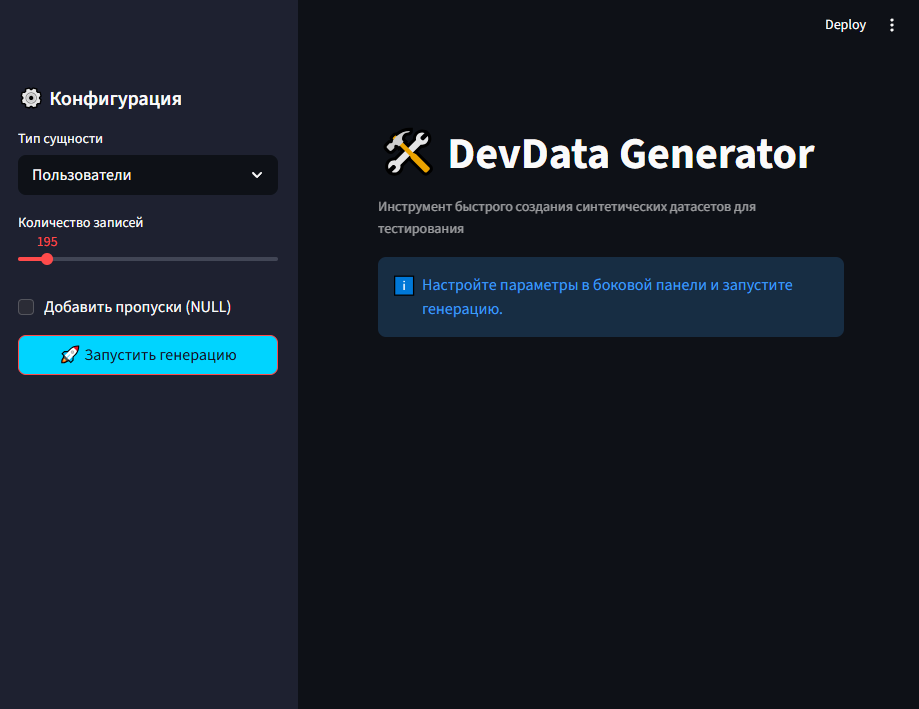
\includegraphics[width=17cm]{4.png}
		\caption{Главный экран дашборда с предпросмотром таблицы}
	\end{figure}
	\begin{figure}[H]
		\centering
		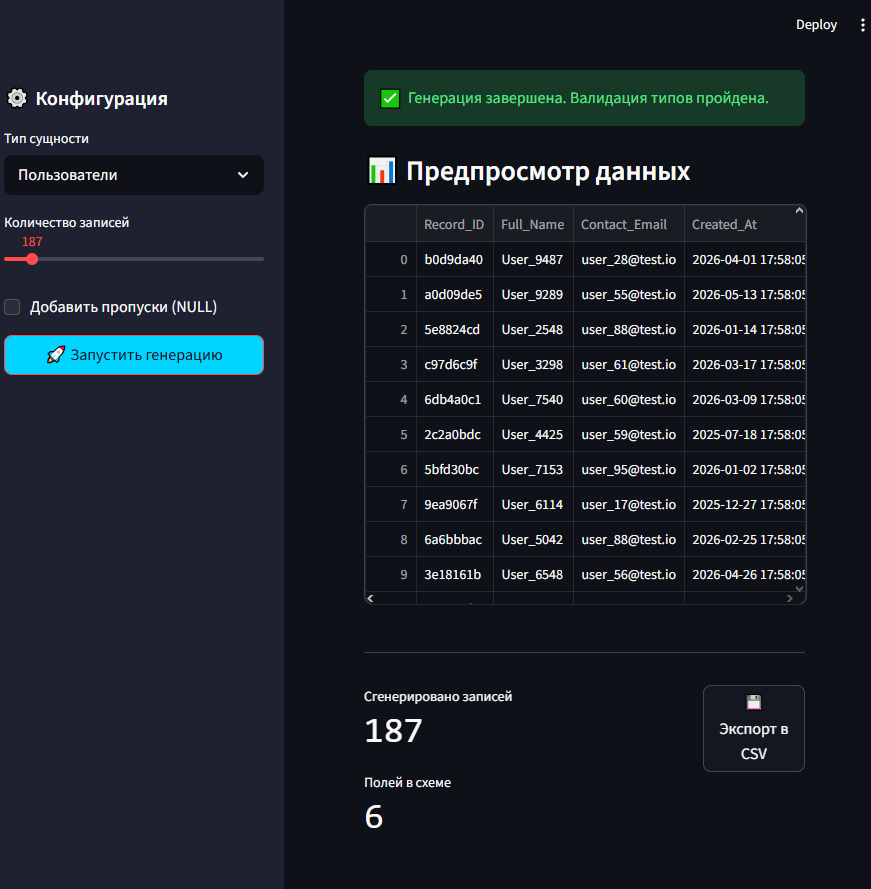
\includegraphics[width=17cm]{5.png}
		\caption{Процесс симуляции ETL-конвейера (st.spinner)}
	\end{figure}
	\subsection*{3.4 Листинг финального кода}
	\lstinputlisting[language=Python]{6.nonutf.txt}
	\newpage
	\section*{Заключение}
	\noindent
	В ходе выполнения лабораторной работы был реализован полный цикл создания MVP DevTools-приложения для генерации тестовых данных с использованием методологии <<быстрого прототипирования>> на основе генеративных моделей.
	\noindent
	\textbf{Оценка моделей:}
	\begin{itemize}
		\item \textbf{DeepSeek Chat} продемонстрировал высокую точность в генерации архитектурных решений и написании рабочего кода на Streamlit/Pandas.
		\item \textbf{DALL-E 3} корректно генерирует технические иконки при указании конкретных Hex-кодов и стилевого направления. Требует явного указания transparent background.
		\item \textbf{Qwen} показал отличные результаты в валидации промптов и поиске логических несоответствий между ТЗ и сгенерированным кодом.
	\end{itemize}
	\noindent
	\textbf{Выявленные ограничения:}
	\begin{enumerate}
		\item Стандартные виджеты Streamlit сложно стилизовать без внедрения custom CSS.
		\item Модели часто игнорируют требование к <<имитации задержки>> без явного указания функции time.sleep() и контекста UX.
		\item При генерации больших таблиц (>2000 строк) требуется явное ограничение предпросмотра (head()), иначе интерфейс зависает.
	\end{enumerate}
	\noindent
	\textbf{Наиболее эффективные техники промпт-инжиниринга:}
	\begin{itemize}
		\item \textbf{Tree of Thoughts} --- анализ архитектурных альтернатив предотвратил выбор избыточных решений и ускорил деплой MVP.
		\item \textbf{Self-Correction Loop} --- скриншотная отладка позволила исправить верстку и логику состояний за 4 итерации без ручного поиска в документации.
		\item \textbf{Chain of Density} --- <<уплотнение смысла>> в ТЗ обеспечило точное соответствие сгенерированного кода требованиям (названия полей, типы данных, структура UI).
	\end{itemize}
	\newpage
	\section*{Приложения}
	\subsection*{Приложение А. Инструкции по запуску}
	\begin{lstlisting}[language=bash]
		pip install streamlit pandas faker
		streamlit run main.py
	\end{lstlisting}
	Откройте браузер по адресу: \url{http://localhost:8501}
	\subsection*{Приложение Б. Ссылки}
	Ссылка на яндекс диск: \url{https://disk.yandex.ru/d/kBvAASygvDpb6A}
	\newpage
	\subsection*{Приложение В. Медиа-материалы}
	\begin{figure}[H]
		\centering
		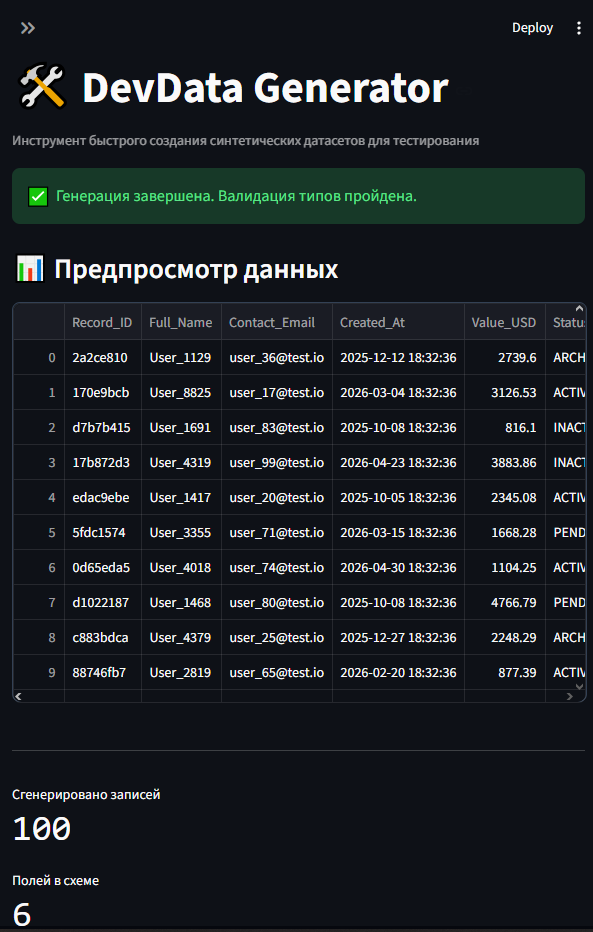
\includegraphics[width=10cm]{6.png}
		\caption{Мобильная адаптация и панель экспорта}
	\end{figure}
\end{document}